\documentclass[twocolumn,prb,showpacs,superscriptaddress]{revtex4}
\usepackage{graphicx}

%
% warning: if you redefine \r you will have troubles with the angstrom,
% which is internally defined as \r{A}
%

\def\k{{\bf k}}

% -------
\usepackage{soul}
\usepackage{color}
\definecolor{yellow}{rgb}{1,1,0}
\definecolor{lightblue}{rgb}{0.6,0.6,0.9}
\sethlcolor{yellow}
% -------

\begin{document}

\title{GW method using density-functional perturbation theory}

\author{Feliciano Giustino}
\email{feliciano.giustino@materials.ox.ac.uk}
\affiliation{Department of Materials, University of Oxford, Parks Road, Oxford OX1 3PH, United Kingdom}
\affiliation{Department of Physics, University of California at Berkeley, 
Berkeley, California 94720, USA,
and Materials Sciences Division, Lawrence Berkeley National Laboratory, 
Berkeley, California 94720, USA}
\author{Marvin L. Cohen}
\author{Steven G. Louie}
\affiliation{Department of Physics, University of California at Berkeley, 
Berkeley, California 94720, USA,
and Materials Sciences Division, Lawrence Berkeley National Laboratory, 
Berkeley, California 94720, USA}
\date{\today}

\begin{abstract}
We propose a new approach to quasiparticle GW calculations based on the
direct evaluation of the Green's function and of the screened Coulomb interaction.
The Green's function is computed by using Haydock's recursion method,
and the screened Coulomb interaction is computed using density-functional
perturbation theory. The frequency dependence is explicitely calculated,
without resorting to the plasmon pole approximation. We implemented the
proposed method within the empirical pseudopotential formalism and 
studied silicon as a test case. We discuss the advantages of our method
over existing approaches and future plans.
\end{abstract}

\pacs{71.15.-m, % Methods of electronic structure calculations
      71.15.Qe} % Excited states: methodology

\maketitle

\section{Introduction}

Importance of GW calculations, Motivation, History of the idea,
Explanation of where we are and how the manuscript is organized.

\section{Methodology overview}

\section{Green's function}

\section{Screened Coulomb interaction}

\section{Implementation}

The approach described above is currently implemented in the empirical
pseudopotential code {\tt OxfordGW}. 

\section{Results}

\section{Conclusions and outlook}

\begin  {figure}
\begin  {center}
%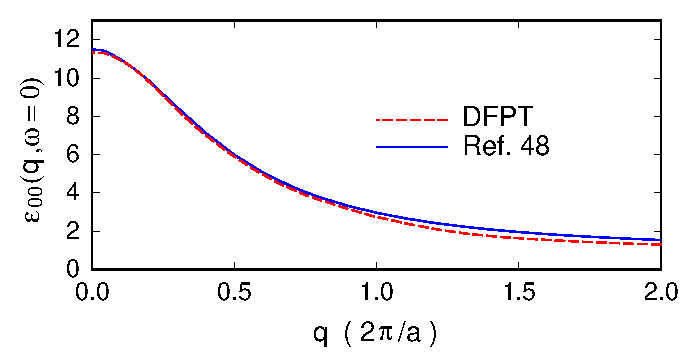
\includegraphics[width=7.5cm]{fig1.eps}
\end    {center}
\caption{\label{fig1} 
        ciao
        }
\end    {figure}

\begin{acknowledgments}
Computational resources were provided by the Oxford Supercomputing Centre.
This work was partly supported by the National Science Foundation Grant No. DMR04-39768 and by
the Director, Office of Science, Office of Basic Energy Sciences, Materials Sciences
and Engineering Division, U.\ S.\ Department of Energy under Contract No. DE-AC02-05CH11231.
\end{acknowledgments}

\appendix

\section{Scaling properties}

\begin{thebibliography}{99}

\bibitem{hl}
L. Hedin and S. Lundqvist,
Effects of the electron-electron and the electron-phonon interaction in
the one-electron states of solids,
in {\it Solid State Physics}, ed. by F. Seitz, D. Turnbull, and
H. Ehrenreich, (Academic, New York, 1969), vol.\ 23, pag. 1.

\end{thebibliography}

\end{document}
